%!TEX root = ../thesis.tex
%*******************************************************************************
%****************************** Second Chapter *********************************
%*******************************************************************************

\chapter{Heavy Neutral Leptons}

\ifpdf
    \graphicspath{{Chapter2/Figs/Raster/}{Chapter2/Figs/PDF/}{Chapter2/Figs/}}
\else
    \graphicspath{{Chapter2/Figs/Vector/}{Chapter2/Figs/}}
\fi

%********************************** %Opening  **************************************

Chapter 2 Opening

%********************************** %First Section  **************************************
\newpage
\section{Right-Handed Heavy Neutral States}

%Motivation for HNL theory: neutrino oscillation -> right handed Dirac mass term
%TODO: Ref more neutrino experiments
The discovery of neutrino oscillation has been well established by the Super Kamiokande collaboration in 1998 \cite{} and the SNO collaboration in 2001 \cite{}. 
The neutrinos can convert from one flavour to another and therefore, clearly indicates the existence of non-zero mass.
However, there is currently no mass generation mechanism for neutrinos in the Standard Model (SM).
Experiments have found neutrinos to be left-handed \cite{} and thus, cannot couple with the Higgs boson to acquire any mass.

%RH Mass mechanism i.e. Dirac mass term
This motivates an introduction of a right-handed neutral counterpart to the neutrinos, such that the Dirac mass term resulting from the Yukawa coupling to the Higgs field can be constructed using the same Lagrangian recipe as all other SM particles
\begin{equation}
\mathcal{L}^{Dirac} = -m_{D}(\overline{\nu}_{L}\nu_{R} + h.c.)
\end{equation}
where the Dirac mass is $m_{D} = Yv/\sqrt{2}$, the Yukawa coupling is $Y$, the Higss vacuum expectation value is $v$, the right and left-handed neutrino fields are $\nu_{R}$, $\nu_{L}$ respectively and $h.c.$ is the hermitian conjugate.

%Majorana Mechanism
Due to the neutral nature of the neutrinos, an additional solution to the Dirac Lagrangian is available, as proposed by Ettore Majorana in 1937 \cite{}.
While the Dirac mass requires the existence of a right-handed neutrino state, Majorana constructed a new mass term using exclusively the left-handed chiral state.
The right-handed component can be written in terms of the left-handed component as $\nu^{C}_{L}=C\overline{\nu_{L}}^{T}$, where $C$ is the charge conjugation operator.
In this case, the Dirac mass term does not exist and the neutrino Lagrangian can only contain the Majorana mass term as following
\begin{equation}
	\mathcal{L}^{Majorana} = -\frac{1}{2}m_{M}(\overline{\nu}_{L}\nu_{L}^{C} + h.c.)
\end{equation}
where $m_{M}$ is the theorised Majorana mass. 
The factor of a half is introduced to account for double counting since the hermitian conjugate is identical.

%Motivation of large mass
Thus, the right-handed neutrinos provide a mass generation mechanism for the SM (or active) neutrinos via either Dirac or Majorana mass terms.
Moreover, for having masses $\gg$ eV , the new particles can explain the extreme light mass of the active neutrinos via the See-saw mechanism \cite{}.

%Larger mass than eV neutrino --> Heavy Neutral Lepton
%HNL characteristisc: no charge, mass mixing, weaker-than-weak
The neutral nature of the right-handed neutrinos require all the SM charges to be zero and therefore, will not interact directly via the strong, electromagnetic or weak forces.
The only possible interaction is via mass mixing with the active neutrinos \cite{}.
These weaker-than-weak right-handed particles are often referred in text as \textit{sterile neutrinos}.
Since their masses are significantly massive compared to the active neutrinos, this also gains them the name \textit{Heavy Neutral Leptons} (HNLs), which will be used in this thesis.

%PMNS matrix mixing
From a generic phenomenological approach, HNLs can be added to the SM by extending the Pontecorvo-Maki-Nakagawa-Sakata (PMNS) matrix.
The PMNS matrix describing the mixing of the SM neutrino flavour eigenstates, $\nu_{\alpha}$ ($\alpha=e,\mu,\tau$) and the mass eigenstates $\nu_{i}$ ($i=1,2,3$) is
\begin{equation}
	U_{PMNS} =
	\begin{pmatrix}
		U_{e1} & U_{e2} & U_{e3}\\
		U_{\mu1} & U_{\mu2} & U_{\mu3}\\
		U_{\tau1} & U_{\tau2} & U_{\tau3}\\
	\end{pmatrix}
\end{equation}
The flavour eigenstates $\nu_{\alpha}$ undergo weak interaction whilst the mass eigenstates $\nu_{i}$ describe the neutrino propagation in space and time.
For an addition of a single HNL with mass $m_{N}$, the PMNS can be extended to describe the mass mixing between the SM neutrinos and a heavy eigenstate $N$ as 
\begin{equation}
	U_{PMNS}^{Extended} =
	\begin{pmatrix}
		U_{e1} & U_{e2} & U_{e3} & U_{e4}\\
		U_{\mu1} & U_{\mu2} & U_{\mu3} & U_{\mu4}\\
		U_{\tau1} & U_{\tau2} & U_{\tau3} & U_{\tau4}\\
		U_{N1} & U_{N2} & U_{N3} & U_{N4}\\
	\end{pmatrix}
\end{equation}
where the index 4 is reserved for the newly added $N$.
Then, the flavour eigenstates  $\nu_{\alpha}$ of the SM neutrinos can be written as the linear combination of the mass eigenstates $\nu_{i}$ and the HNL eigenstate $N$ as  
\begin{equation}
	\nu_{\alpha}=\sum U_{\alpha i}\nu_{i} + U_{\alpha 4}N
\end{equation}
where $U_{\alpha i }$ ($i=1,2,3$ and $\alpha=e,\mu,\tau$) are the elements of the PMNS matrix.

%Available mass range 
The mass range of the HNLs can span over many orders many orders of magnitudes and the number of HNLs are unconstrained.
Different theoretical models of HNLs have been developed and a comprehensive review has been discussed, see Ref. \cite{}. 
In this thesis, the existence of HNLs will be explored in a minimal way, assuming an addition of a single HNL to the SM.  
The HNL mass range of interest must be able to be produced from the Booster Neutrino Beam (BNB) and directly detected by the Short-Baseline Near Detector (SBND), which limits the mass to $m_{N}=\mathcal{O}$(100 MeV).
At this mass range over the baseline distance of 110 m, oscillation with the active neutrinos results in coherence loss \cite{}.
Instead, the HNLs are expected to travel over a long distance before decaying into SM observables via mass mixing.

%This thesis: simple phenomenological model
%Example model: minininal neutrino extension of the SM
%The HNLs have been predicted by many different models, where a comprehensive overview has been discussed here \cite{}.
%A particular model requires a minimum extension to the SM has been presented, \textit{Neutrino Minimal Extension of the SM} ($\nu$MSM)\cite{}.
%The model introduces three generations of HNLs.
%The two heavier ones N$_{1,2}$ in the mass range of $\mathcal{O}$(10 GeV) and $\mathcal{O}$(100 MeV) can generate the mass of the active neutrinos via the See-saw mechanism, whilst the third and lightest N$_{3}$ with keV mass can be a viable dark matter candidate.
%$\nu$MSM also accounts for the currently observed matter-antimatter asymmetry for having the heavy HNLs oscillating in a charge and parity violating manner during the early universe, dubbed leptogenesis via neutrino oscillations. 
 
\section{Production}

%Decay mechanism: replace SM with a HNL -> mixing angle
In any neutrino-producing processes, HNLs can be produced in substitute of neutrinos with a rate proportional to $|U_{\alpha4}|^{2}$ if kinematically allowed. 
This means that HNLs can be produced via meson decays, which can be probed experimentally.
An example diagram of such decay is depicted in Fig. \ref{fig:kaonDiagram}, showing a two-body decay of a charged kaon into a muon with either an active neutrino or a HNL.

\begin{figure}[htbp!]
%\hfill
\begin{subfigure}[h]{0.4\linewidth}
\centering    
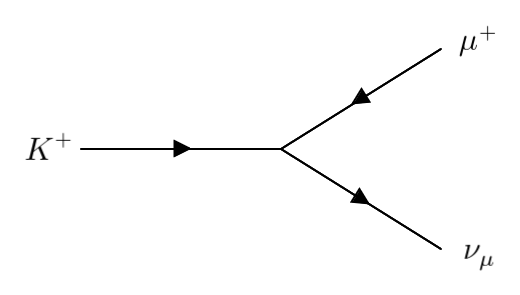
\includegraphics[width=\linewidth]{K_to_nu}
\caption{}
\end{subfigure}
\hfill
\begin{subfigure}[h]{0.4\linewidth}
\centering    
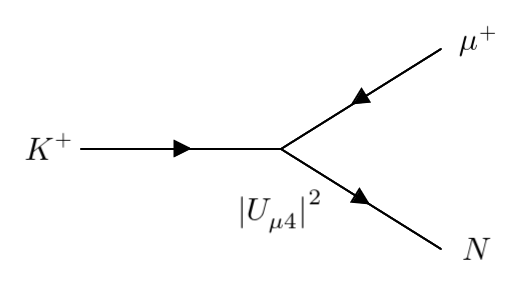
\includegraphics[width=\linewidth]{K_to_HNL}
\caption{}
\end{subfigure}%
%\hfill
\caption[kaonDiagram]{
Diagrams for the production of an active neutrino (a) and a HNL mediated by $|U_{\mu4}|^{2}$ (b) from a two-body decay of a charged kaon.
}\label{fig:kaonDiagram}
\end{figure}

%HNL from BNB beam
%TODO: add rho function to appendix
HNLs can be probed directly via meson decay produced from the BNB beam.
The dominant production channel of the HNL flux comes from charged kaon decays, whilst the contributions from charged and neutral pion decays are negligible. 
In general, the branching ratio of a two-body charged kaon decay into a HNL can be expressed as 
\begin{equation}
	Br(K^{+}\rightarrow l^{+}_{\alpha}N) = Br(K^{+}\rightarrow l^{+}_{\alpha}\nu_{\alpha})\left(\frac{|U_{\alpha 4}|^{2}}{1 - |U_{\alpha 4}|^{2}}\right)\rho_{N}\left(\frac{m^{2}_{l_{\alpha}}}{m^{2}_{K}}, \frac{m^{2}_{N}}{m^{2}_{K}} \right) 
\end{equation}
where $Br(K^{+}\rightarrow l^{+}_{\alpha}\nu_{\alpha})$ is the two-body branching ratio into SM neutrinos and $\rho_{N}$ is a kinematics factor accounting for the available phase space in the decay \cite{}. The complete expansion of the function $\rho_{N}$ is as following

\begin{equation}
	\rho_{N}(x,y) = \frac{(x+y-(x-y)^{2})\sqrt{1+x^{2}+y^{2}-2(x+y+xy)}}{x(1-x)^{2}}
\label{eq:KinematicsFactor}
\end{equation}


The available phase space of the HNL is constrained by the mass of the charged kaon.
Since the mass of a charged kaon ($m_{K} = 494 $ MeV) is smaller than the mass of a tau ($m_{\tau}=1777 $ MeV), $\tau$-flavour leptons cannot be produced from the decay.  
This means the final state leptons can be either electrons and muons, which determines the flavours of the mixing angle $|U_{\alpha4}|^{2}$ that can be probed to be $\alpha = e, \mu$.
The two-body decay of a charged kaon sets the upper limit of the HNL mass such that
\begin{equation}
	m_{N} = m_{K} - m_{l_{\alpha}}
\end{equation}
where, $m_{e}= 0.511 $ MeV and $m_{\mu}= 106 $ MeV.
Therefore, the maximum mass $m_{N}$ can be probed is $\sim493$ MeV  and $\sim388$ MeV via the mixing angle $|U_{e4}|^{2}$ and $|U_{\mu4}|^{2}$ respectively.

%Helicity Unsuppression i.e. K ->Ne and K->Nmu
%Enahancement factor??
%TODO: describe the plots
Furthermore, helicity suppression that occurs in the case of mesons decaying into a SM neutrino has minimal effects in the same case of HNLs due to HNLs being massive \cite{}.
The contribution from helicity suppression can be greater than one compared to the neutrino production, which indicates helicity \textit{enhancement} in the HNL production.
The kinematics factor $\rho_{N}$ from Eq. \ref{eq:KinematicsFactor}, also accounting for this enhancement in the available phase space, is plotted against the mass of HNLs as shown in Fig. \ref{fig:KinematicsFactor}.
Significant enhancement can be seen for the rate of $K^{+}\rightarrow e^{+}N$ by a factor of $10^{5}$.
For the production of HNL of interest from the BNB beam, the kinematics factor for the $K^{+}\rightarrow \mu^{+}N$ channel varies between 1.5 and 4.

\begin{figure}[htbp!] 
\centering    
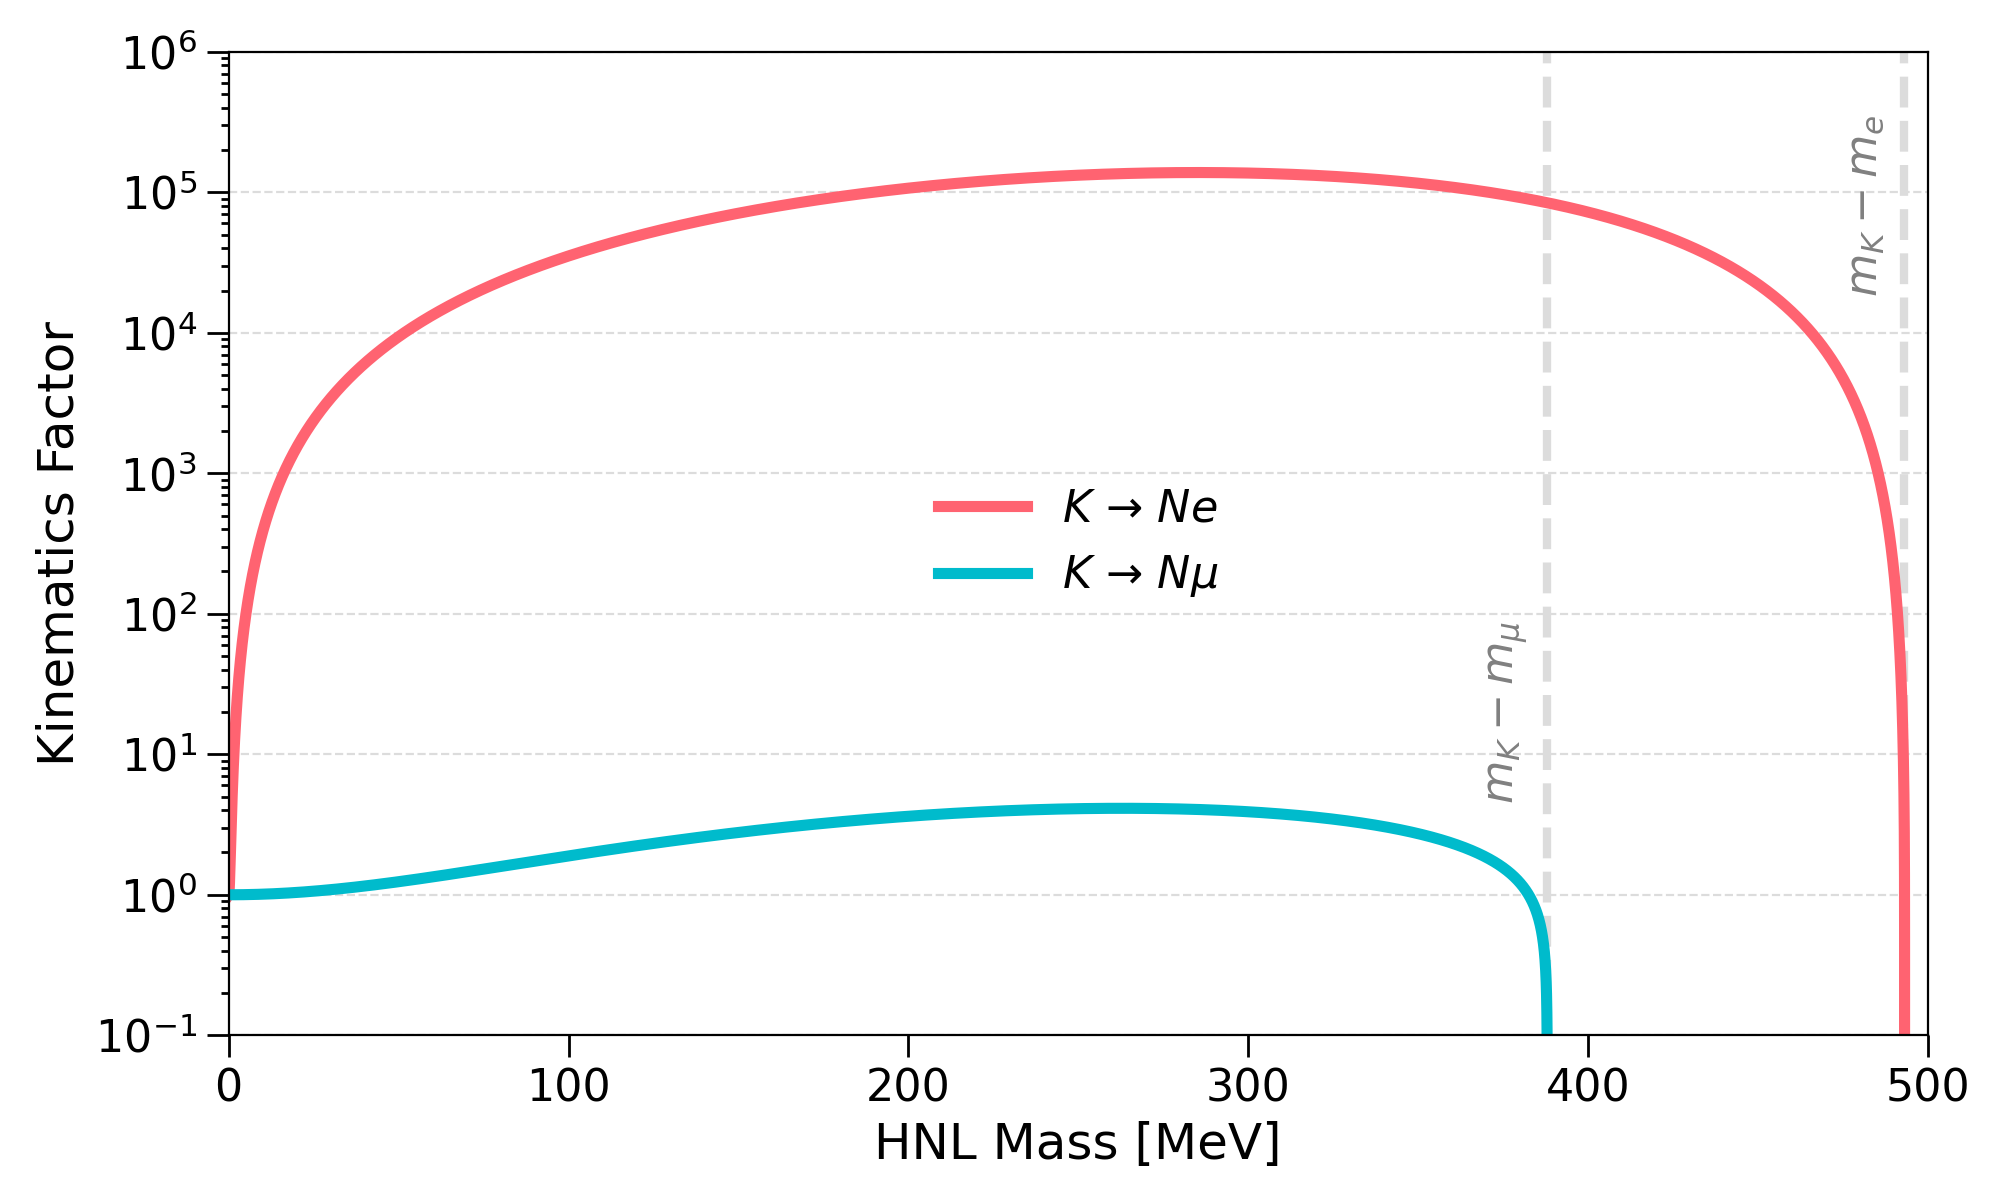
\includegraphics[width=1.0\textwidth]{kinematics_factor}
\caption[KinematicsFactor]{
Kinematics factor of HNL production rate from meson decays compared to analogous SM neutrino production, given by function $\rho_{N}$ from Eq. \ref{eq:KinematicsFactor}.
The pink line shows the enhancement associated with the production from kaons via the mixing angle $|U_{e4}|^{2}$ whilst the blue line shows the enhancement associated with the mixing angle $|U_{\mu4}|^{2}$.
The vertical dashed gray lines indicate limit on the HNL mass from each mixing angle. 
}
\label{fig:KinematicsFactor}
\end{figure}

\section{Decay}

%DIF with coupling
HNLs are unstable particles and therefore decay in flight with a lifetime proportional to the mixing angle $|U_{\alpha4}|^{2}$ $(\alpha=e,\mu,\tau)$, such that HNLs must survive long enough to reach the detector before decaying into observable particles.
Since $|U_{\alpha4}|^{2}$ is the same coupling responsible for the HNL production, the observed event rate at the detector scale with $|U_{\alpha4}|^{4}$.
At the mass $\mathcal{O}$(100 MeV), the tau-flavour mixing angle is kinematically forbidden and thus, the possible decay channels for HNLs are \cite{}

%Possible decay channel
\begin{equation}
\begin{split}
	N\rightarrow e^{-}\pi^{+},\qquad 
	N\rightarrow \mu^{-}\pi^{+},\qquad
	N\rightarrow \nu \pi^{0},\qquad 
	N\rightarrow \nu \gamma,\qquad \\ 
	N\rightarrow \nu e^{-} e^{+},\qquad 
	N\rightarrow \nu \mu^{-} \mu^{+},\qquad 
	N\rightarrow \nu \mu^{-}e^{+},\qquad
	N\rightarrow \nu \nu \nu. 
\end{split}
\end{equation}
In the case of HNLs are Majorana, the charge conjugates for the decays are also available.

%TODO: branching diagram plots
\begin{figure}[htbp!] 
\centering    
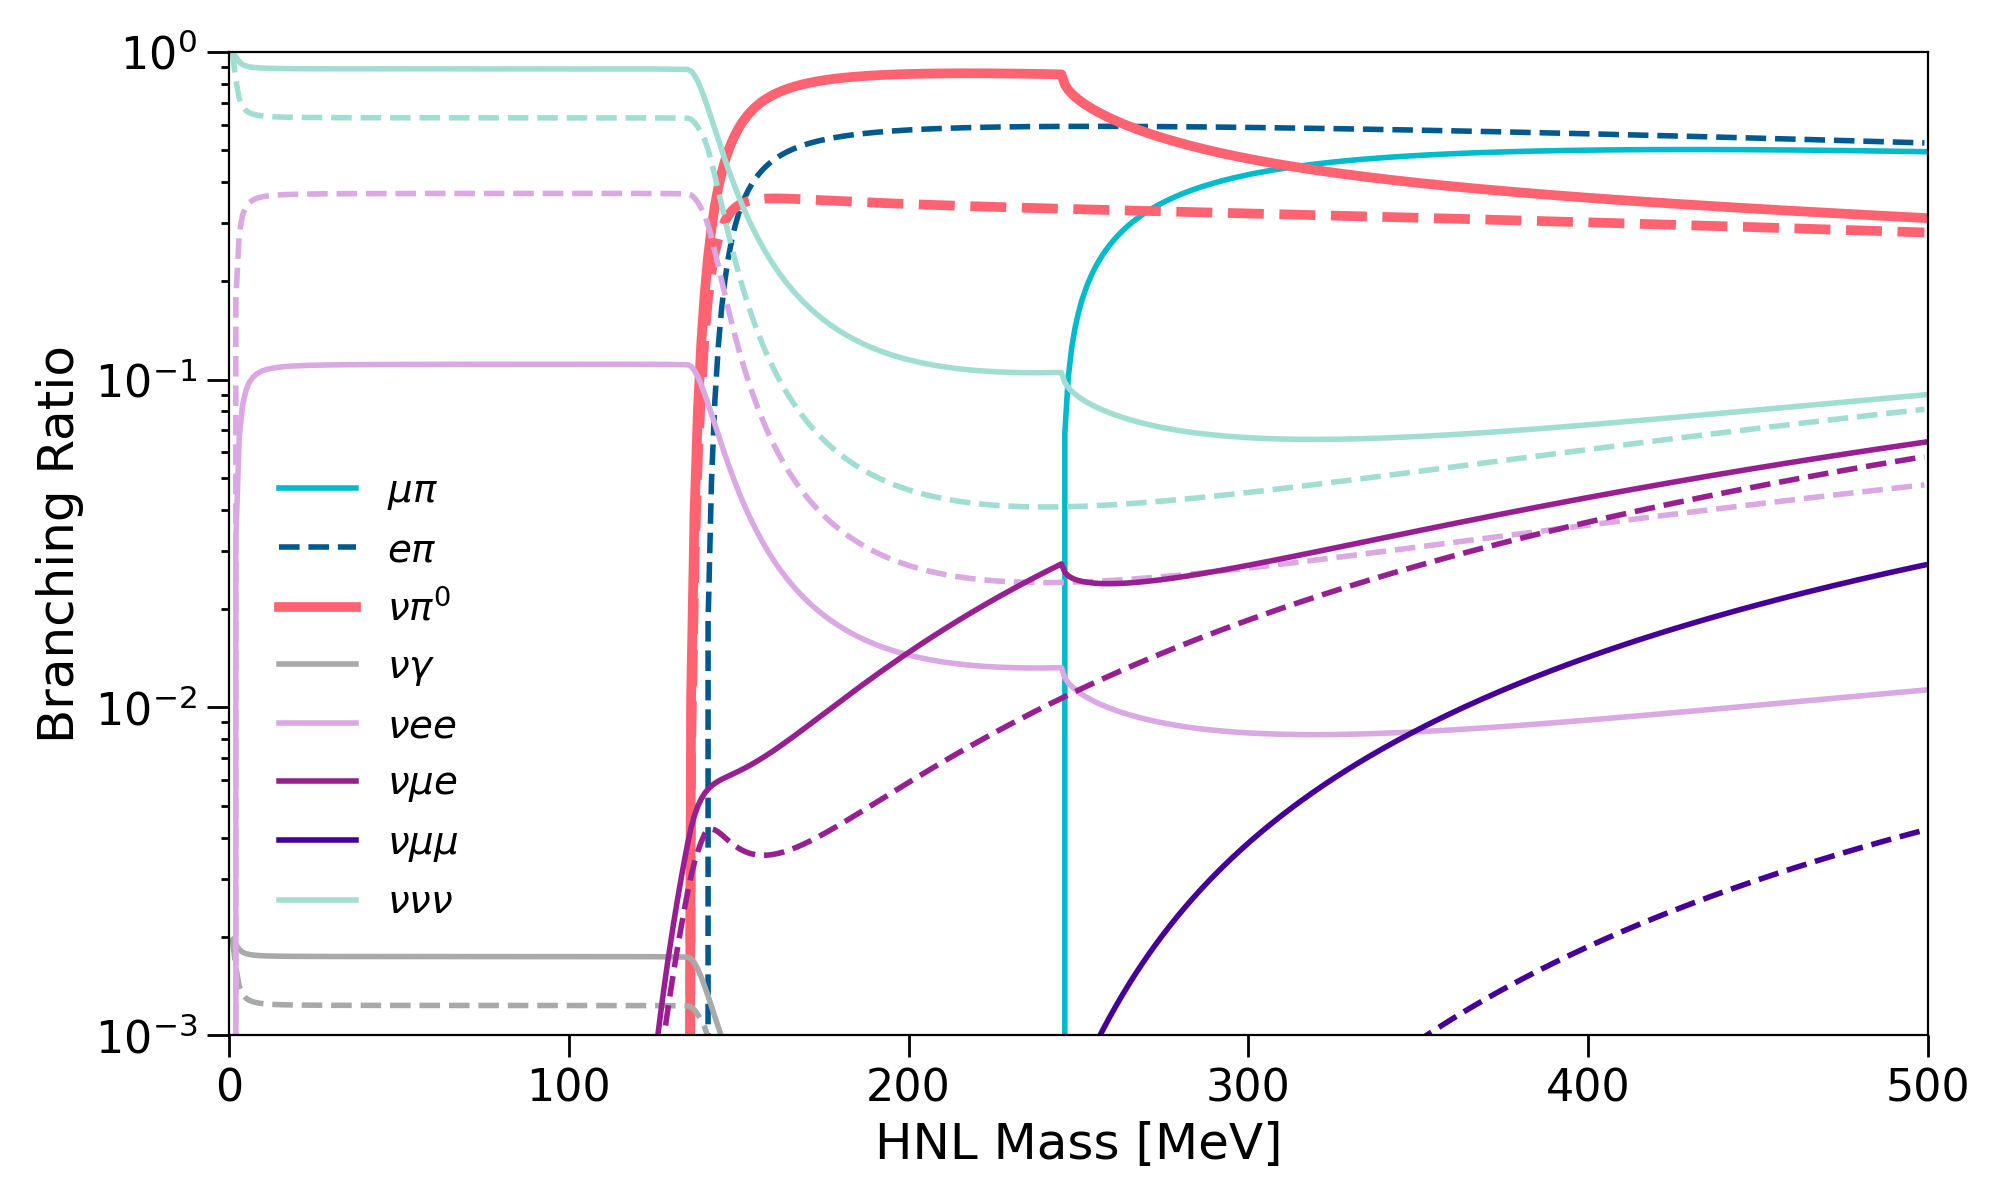
\includegraphics[width=1.0\textwidth]{branching_ratio}
\caption[branching_ratio]{
The branching ratio of decay channels of a Majorana HNL as a function of its mass.
The decay widths of each channel is taken from Ref. \cite{}.
Solid lines are branching ratios via the muon-flavour mixing angle ($[U_{e4}:U_{\mu4}:U_{\tau4}]=[0:1:0]$) and dashed lines are branching ratios via the electron-flavour mixing angle ($[U_{e4}:U_{\mu4}:U_{\tau4}]=[1:0:0]$).
In pink and thicker line width is the decay channel studied in this thesis $N\rightarrow \nu \pi^{0}.$
}
\label{fig:branching_ratio}
\end{figure}

%Overall description of each BR channel
The branching ratio of decay channels for a Majorana HNL is shown in Fig. \ref{fig:branching_ratio}, with decay widths reference taken from \cite {}.
For $m_{N} < 135$ MeV, the branching ratio is dominated by the channel $N\rightarrow \nu\nu\nu$, however is experimentally unobservable.
Whilst the channel $N\rightarrow \nu \gamma$ is highly suppressed, the channel $N\rightarrow \nu e^{-}e^{+}$ provides the best sensitivity at this mass range.
For $m_{N} > 135$ MeV, such that a HNL has sufficient mass to decay into a neutral pion, the channel $N\rightarrow \nu \pi^{0}$ dominates the muon-flavour mixing angle, whilst the channel $N\rightarrow e^{-}\pi^{+}$ dominates the electron-flavou mixing angle.
For $m_{N} > 245$ MeV, equivalent to the mass of a muon and a charged pion combined, the lepton-pion channels are the leading decays. 
Both channels $N\rightarrow \nu \mu^{-}e^{+}$ and $N\rightarrow \nu \mu^{-}\mu^{+}$ are not competitive in relative to all other channels at the same mass value.  

%Desciption on the specific decay channel of thesis: HNL -> nu + pi0
%TODO: what mass range am I looking for.
This thesis searches for the existence of HNL via $N\rightarrow\nu \pi^{0}$, which is the leading channel the muon-flavour mixing angle in the mass range $ 135 < m_{N} < 245 $ MeV.
In the same mass range of the electron-flavour mixing angle, this region has been well-explored.
Therefore, this thesis focuses on non-zero $|U_{\mu4}|$, assuming $|U_{e4}| = |U_{\tau4}| = 0$.  
In this case, the decay width of this channel is modelled as \cite{}:
\begin{equation}
	\Gamma(N\rightarrow \nu \pi^{0}) = \frac{G_{F}^{2}m_{N}^{3}}{32\pi}f^{2}_{\pi^{0}}|U_{\mu4}|^{2}\left(1-\left(\frac{m_{\pi^{0}}}{m_{N}}\right)^{2}\right)^{2}
\label{eq:pi0}
\end{equation}
where $G_{F}$ is the Fermi constant, $f_{\pi^{0}}$ is the decay constant of a neutral pion and $m_{\pi^{0}}$ is the mass of a neutral pion.
It is important to note that this decay width expression has been derived several times in various literature with slightly different variations. 
Eq. \ref{eq:pi0} does not contain an additional factor of 2 in the denominator compared to Ref. \cite{} and \cite{}.
The resulting event rate still agrees within the same order of magnitude.

\begin{figure}[htbp!]
%\hfill
\begin{subfigure}[h]{0.49\linewidth}
\centering    
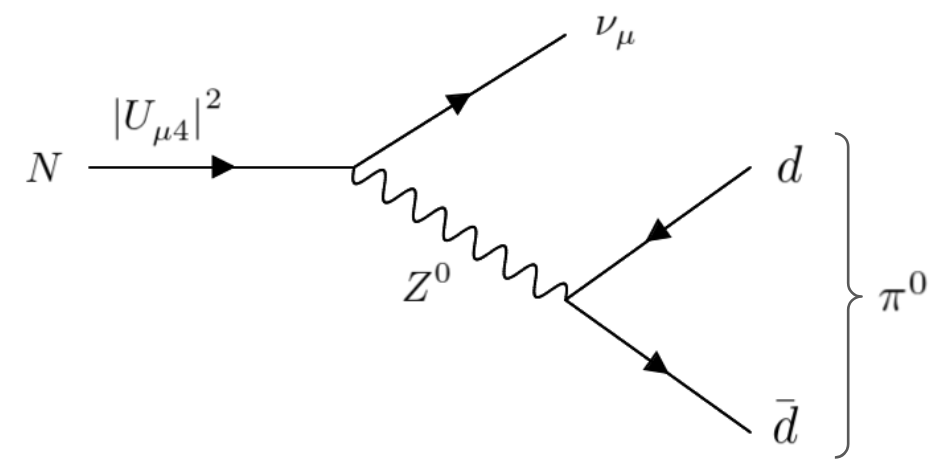
\includegraphics[width=\linewidth]{N_to_pi0_edit}
\caption{}
\end{subfigure}
\hfill
\begin{subfigure}[h]{0.49\linewidth}
\centering    
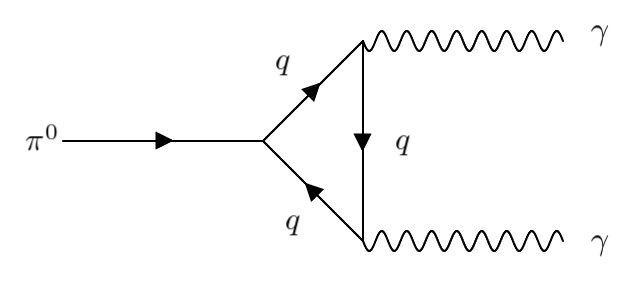
\includegraphics[width=\linewidth]{pi0_to_gam}
\caption{}
\end{subfigure}%
%\hfill
\caption[decayDiagram]{
Diagrams of a HNL decaying into a neutrino and a neutral pion mediated by $|U_{\mu4}|^{2}$ (a) and a neutral pion decaying into two photons (b).
}\label{fig:decayDiagram}
\end{figure}

%Decay signature in TPC
%TODO: neutral pion BR 
Once a HNL decays into a neutrino and a neutral pion inside the detector, the neutrino escapes the detector undetected whilst the neutral pion decays into two photons with a branching ratio of 0.988 \cite{}. 
Diagrams of the decays are shown in Fig. \ref{fig:decayDiagram}.
This decay results into a particular event topology inside a LArTPC: two photon showers originating from the same vertex without any hadronic activities.
Neutral-current neutrino interactions resulting into a neutral pion also share the same final state particles and thus, represent the main background of this search.
However, different event kinematics and precise timing resolution, as detailed in Section \ref{}, provide a good separation between HNL decays and neutrino interactions. 

%Dirac or Majorana Nature
HNLs can be either Dirac or Majorana in nature.
Majorana HNLs would violate the conservation of lepton number, whereas Dirac HNLs would perserves it.
Therefore the expected event rate of Majorana HNLs is double the rate of Dirac HNLs.
Moreover, a Majorana HNL would decay isotropically whilst in the case of a Dirac HNL, the helicity of the produced neutrino would determine the direction of the decay products \cite{}.
Ref \cite{} has demonstrated that a HNL decaying into a neutral meson is isotropic in the rest frame, and thus, does not depend on helicity of the partner neutrino.
This means that the decay channel $N\rightarrow \nu \pi^{0}$ is insensitive to the Dirac nature of HNLs.
This thesis therefore assumes HNLs are Majorana particles for the search.

\section{Previous Experimental Searches}

%Number of fermion families = Z boson decay for LH neutrinos, RH neutrinos is not constrained

%Overview of different types of searches
HNLs have been searched by experiments over the decades, across a large range of mass.
While oscillation experiments and precise $\beta$ decay experiments can probe HNL at the mass range of eV and keV, collider experiments have set limits on on GeV-scale HNLs.
No evidence of HNLs existence has been found, and thus, experiments have set upper limits on to the mixing angle $|U_{\alpha4}|^{4}$ $(\alpha=e,\mu,\tau)$.
The sensitivity limits are often expressed in terms of the mixing angle $|U_{\alpha4}|^{4}$ as a function of the HNL mass.

Here, the existing experimental limits on HNLs of $\mathcal{O}$ (100 MeV) are presented, specifically between $ 0 < m_{N} < 245 $ MeV which is relevant to the final states $\nu\pi^{0}$.
At this mass range, the primary experimental methods are peak searches and decay searches.
Peak searches probe only the production rate of HNL whilst decay searches probe both production and decay rates.

\subsection{Peak Searches}

Peak search experiments measure the energy spectrum of a meson decay that would produce a HNL. 
The leptonic decay of a meson can be modelled as $P\rightarrow l + Invisble$, where $P$ is the parent meson (a pion or a kaon) and $l$ is the daughter particle (a pion or a lepton).
The $Invisble$ decay products are attributed to HNLs and SM neutrinos.
The produced HNLs are expected to exit the detector before decaying whilst the SM neutrinos can also escape before interacting, which act as the main background of the search.
Since the momenta of $P$ and $l$ can be precisely measured, the missing invariant mass can therefore be derived from the momenta as $m^{2}_{miss} = (P_{p} - P_{l})^{2}$, where $P_{p}$ and $P_{l}$ are the parent and daughter 4-momentum.
Given that the neutrinos are nearly massless, the mass of the HNL can be treated as $m_{HNL} = m_{miss}$ and an excess over background will be presence at $m_{miss}$.

To infer the sensitivity contour, the flavour of the lepton $l$ determines the flavour of the coupling whilst the amplitude of the decay spectrum at $m_{miss}$ determines the upper limit on the coupling.
Limited placed by the peak search experiment are independent of whether the HNL is Dirac or Majorana since it does not affect the kinematics of the meson decay.
For $|U_{\mu4}|^{2}$, the most competitive limits have been set by the following experiments, on pion and kaon decay spectrum:


\subsubsection{Pion Decay Spectrum Peak Searches}

\begin{coloritemize}
\item \textbf{SIN} (Swiss Institute for Nuclear Research) performed a peak search using stopped positive pions decay via $\pi^{+} \rightarrow \mu^{+} + Invisible$, using a scintillator in 1981 and a germanium detector in 1987.
The pion enables probing HNLs in the low mass range of $\mathcal{O}$(10 MeV).
Upper limits of $|U_{\mu4}|^{2}$ were placed in the mass range 1--30 MeV at $10^{-5}$ \cite{SIN1, SIN2, SIN3}.

\item The \textbf{PIENU} collaboration at TRIUMF \cite{PIENU} also searched for HNLs using stopped pions.
The most recent result in 2019 set the most stringent limits on $|U_{\mu4}|^{2}$ in the range $10^{-6}$--$10^{-5}$ in the mass range of 15--34 MeV, extending beyond result reported by SIN.

\end{coloritemize}

\subsubsection{Kaon Decay Spectrum Peak Searches}

\begin{coloritemize}
\item The \textbf{KEK} collaboration conducted an experiment called E89 to search for HNLs using the muon range spectrum from stopped kaon decay in 1981--1982. Experiment E104 in 1983 was carried subsequently with improved momentum resolution and background supression.
The kaons were produced using a 0.5 GeV proton beam and $3 \times 10^{6}$ muons from kaon decay were analysed using magnetic spectrograph.
The results from E89 constrained the limits of $|U_{\mu4}|^{2}$ in the range of 10$^{-4}$--10$^{-6}$ for the HNL mass between 70--300 MeV.
The combined results from E89 and E104 furthered the sensitivity towards the lower mass range between 45--300 MeV, however currently unpublished \cite{KEK1, KEK2, KEK3}.

\item The \textbf{E949} collaboration at Brookhaven National Laboratory performed a kaon decay experiment using 21.5 GeV protons in 2002.
The analysis on the decays of $2 \times 10^{21}$ stopped kaons resulted in the limits on $|U_{\mu4}|^{2}$ for the range of mass between 175--300 MeV at the level 10$^{-7}$--10$^{-9}$ \cite{E949}.
\item The \textbf{NA62} collaboration is a kaon decay experiment at the CERN super proton synchrotron.
The collaboration analysed $10^{8}$ stopped kaons from 400 GeV protons extracted from the synchrotron.
The first results, using data set in 2015, placed the upper limits on $|U_{\mu4}|^{2}$ in the range of 10$^{-7}$--10$^{-6}$ for HNL mass in the range 250--373 MeV.
Updated results using a larger dataset collected in 2016--2018 improved the coupling limits by an order of magnitude to 10$^{-8}$--10$^{-7}$ and extended the mass range to 250--384 MeV \cite{NA62A, NA62B}.
\end{coloritemize}

\subsection{Decay Searches}

Decay searches look for decay products of the HNLs.
The HNLs are typically produced outside of the detector before reaching it, potentially decaying into observable SM particles within the detector.
Different combinations of production and decay channel yield distinct expected event rates and therefore, can probe different sensitivity regions associated with different mixing angles.
Decay searches have been historically performed in beam-dump experiments, which are explicitly designed to suppress the background from SM interactions in order to search for rare decay processes.
Recently, modern neutrino experiments with improved resolution can function as competitive beam-dump experiments alongside their neutrino physics programme.
For $|U_{\mu4}|^{2}$, the most competitive limits have been set by the following experiments:

\begin{coloritemize}
%TODO: PS191 Check with David Marsden
\item The CERN \textbf{PS191} experiment was conducted in 1984 with an exposure of 19.2 GeV protons on a beryllium target, resulting in $10^{19}$ POT.
The detector was located at 128 m from the target at an off-axis angle of $2.3^{\circ}$ with respect to the beam direction.
It was designed specifically to search for HNLs by maximising the signal rates and minimising the background rates.
The 216 m$^{3}$ volume (12 m long and a cross-sectional area of 18 m$^{2}$) was filled with helium.
The sparse medium minimises the background rate coming from the SM neutrino interactions whilst the large volume provides a high rate of HNL events. 
Limits were set in the mass range 120--350 MeV for $|U_{\mu4}|^{2}$ in the range of 10$^{-5}$--10$^{-9}$ \cite{PS191A, PS191B}.
	
\item The \textbf{T2K} collaboration recently searched for HNLs using the near detector ND280, located 280 m from the beam target at an off-axis angle of $2.04^{\circ}$.
The analysis was performed on the data collected from 2010-2017, with a beam intensity of 30 GeV proton on graphite target and an exposure of $\approx 2 \times 10^{21}$ POT.
The search was limited to the three argon gas TPC volumes, which minimised the neutrino background rate due to the low gas density.
The results constrained the limits of $|U_{\mu4}|^{2}$ in the range of 10$^{-8}$--10$^{-9}$ for the HNL mass between 250--380 MeV \cite{T2KHNL}.
%The T2K collaboration has also presented results on $|U_{\mu4}|$ in the case where $|U_{e4}|$ and $|U_{\tau4}|$ are assumed to be non-zero and marginalised using results from other channels.

\item The \textbf{NuTeV} collaboration at Fermilab conducted the search for HNLs in 1996 using a high energy neutrino beam produced by protons accelerated from the Tevatron ring.
The dataset consisted of $3 \times 10^{18}$ POT exposure with an energy of 800 GeV.
HNLs were produced from the $D$ mesons produced from protons colliding with the target.
This allowed the HNL mass to reach up to 2000 MeV, surpassing any other beam-dump experiments described here.
The limits on $|U_{\mu4}|^{2}$ in the range 10$^{-6}$--10$^{-7}$ were placed in the mass range of 225--2000 MeV \cite{NuTeV}.

\item The \textbf{MicroBooNE} collaboration presented the first HNLs search using a LArTPC in 2020, followed by two more publications in 2022 and 2023.
The first analysis was performed on data collected from $2 \times 10^{20}$ POT from the on-axis BNB beam, using a delayed trigger to identify HNLs arriving at the detector after the SM neutrino background.
This produced a limits on $|U_{\mu4}|^{2}$ in the range (4.7--0.7)$\times 10^{-7}$ for HNL masses between 260--385 MeV.
The latter two searches focused on HNLs coming from kaons decays in the NuMI absorber, which would enter the detector at an angle to the BNB beam neutrino.
The dataset comprised of two runs with an exposure of $2 \times 10^{20}$ and $5.01 \times 10^{20}$ POT.
The combined results is made of multiple HNL decay channels, probing a wide mass range between 10--385 MeV.
This currently set the most stringent limits on $|U_{\mu4}|^{2}$ in the range 10$^{-2}$--10$^{-8}$ for low MeV-scale HNLs, extending the results from 2019.
\cite{uboone1, uboone2, uboone3}

\end{coloritemize}

%TODO: PLOT of ALL experiments limits!!
